\chapter{Referencial Teórico}
    A fim de encontrar a semelhança entre os códigos, \citeonline{Yin:2015}
    utilizou a Árvore de Sintaxe Abstrata (AST) - estrutura de dados em árvore
    utilizada para representar um bloco de código a partir da análise sintática,
    armazenando símbolos não-terminais nos nós filhos e símbolos terminais nos
    nós folha - para representar um bloco de código. Após a criação das árvores,
    é necessário o uso de métricas para verificar a similaridade entre as árvores.
    Desta forma, foi utilizada a Distância de Edição de Árvore (TED) – ao comparar
    duas árvores, verificam-se quais são as movimentações (inserção, movimentação
    e remoção) necessárias para que as árvores fiquem iguais. Assim, foi
    selecionado a TED normalizado que utiliza estrutura \textit{top-down}:
    quanto mais próximo do nó raiz, maior sua importância. Sua escolha ocorreu
    pelo fato do TED normalizado possuir maior índice na qualidade de agrupamentos.
    
    Os autores do artigo analisado utilizaram os algoritmos de classificação
    DBSCAN e OPTICS para agrupar os códigos semelhantes, visto que obtiveram
    a maior pontuação de silhueta que verifica a distância entre pares dentro
    do agrupamento e entre os agrupamentos. Quanto maior sua pontuação, melhor
    a qualidade do \textit{cluster}. Conforme a Figura \ref{fig:t-SNE}, para
    visualizar os agrupamentos foi utilizado o t-SNE – técnica de redução
    dimensional não linear que preserva a estrutura local dos dados.
    \begin{figure}[ht]
        \centering
        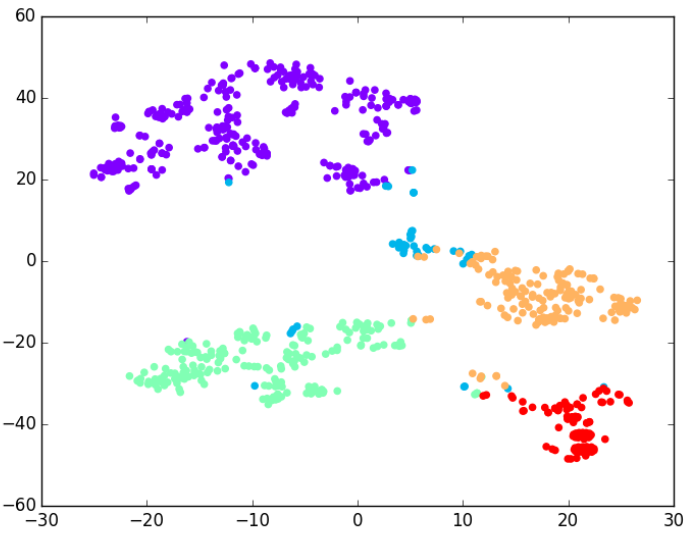
\includegraphics[scale=0.5]{imagem/visualizacao-tSNE.png}
        \caption{Visualização t-SNE. Identificação de quatro grupos: roxo, verde,
        	laranja e vermelho. Os pontos azuis não obtiveram similaridade
        	suficiente para formar um agrupamento ou serem classificados em
        	outro agrupamento. Os agrupamentos foram identificados na semelhança
        	dos códigos. Todas as implementações possuem a função \textit{combine\_anagrams}
        	que possui a variável \textit{words} como parâmetro: no grupo vermelho,
        	essa função possui 3,7 linhas; no agrupamento roxo, 10.9 linhas; no
        	grupo laranja, a função possui 12.5 linhas; e no agrupamento verde,
        	a solução possui 21,3 linhas.}
        \label{fig:t-SNE}
    \end{figure}

    
    Em \citeonline{Glassman:2014}, foi proposto o agrupamento hierárquico de dois
    níveis. No nível mais alto ocorre o particionamento das soluções ao longo do
    plano de separação, considerando apenas características abstratas, como:
    posição da declaração de condicional em relação a declarações de laço de
    repetição (antes, dentro ou depois), profundidade de um laço de repetição
    (\textit{loop}) aninhado, números de nós AST e declarações de retorno,
    \textit{loops} e comparações, por exemplo.
    
    Dentro de cada agrupamento de alto nível, tem um subagrupamento, destinado a
    capturar a dimensão generalizada, construções de linguagem de baixo nível e
    bibliotecas utilizadas. Os agrupamentos internos são formados por meio de 48
    características concretas: operações aritméticas e lógicas, laços de repetição,
    funções de bibliotecas, declarações de atribuição, \textit{loops}, condicional,
    número de variáveis e valores constantes, por exemplo.
    
    \citeonline{Glassman:2014} utiliza o classificador \textit{K-means} para agrupar
    as implementações dos estudante. Foi utilizado diversos valores para \textit{k}
    e a validação dos agrupamentos ocorreu por meio da comparação dos \textit{clusters}
    criado pelo algoritmo de classificação com o que foi criado pelos
    \textit{teaching assistants} (TA). Para os TAs foi entregue 50 códigos
    dos estudantes randomicamente e notou-se que eles ignoraram características
    de baixo nível.
    
    Estes utilizaram a métrica Informação Mútua Ajustada (AMI) - cálculo
    probabilístico - para comparar os agrupamentos dos TA's com cada agrupamento
    gerado pelo \textit{k-means}. Quando o valor de AMI é 0 (zero), quer dizer
    que os agrupamentos são independentes, entretanto, se for igual a 1, indica
    perfeita concordância entre os \textit{clusters}. Quando \textit{k} tinha um
    valor maior ou igual a 15, os agrupamentos do classificador concordaram com
    o agrupamento de cada \textit{teaching assistants}, conforme medição do AMI.
    
    Em \citeonline{Taherkhani:2012}, testou-se a ferramenta Aari para cinco tipos
    de métodos de ordenação: \textit{bubble sort}, \textit{insertion sort},
    \textit{selection sort}, \textit{mergesort} e \textit{quicksort}. Os
    algorítimos classificados como \textit{Others} na Figura \ref{fig:clusterManual}
    é referente ao \textit{shellsort}, \textit{heapsort} e um algoritmo híbrido de
    \textit{quicksort} com \textit{selection sort}. Os autores separaram as
    características em três categorias: características numéricas, características
    descritivas e outras características.
    
    A categoria características numéricas possui o seguinte conjunto de características:
    número de declarações de atribuição; linha de código; complexidade McCabe; total de
    operadores; total de operadores; total de operandos; número de operadores único;
    número de operando único; total do número de operadores e operando; total do
    número de operadores e operando único; número de variáveis; número de laços de
    repetição; número de laços aninhados e número de bloco. Essa característica
    extrai tudo que pode ser medido como inteiro.
    
    Enquanto a categoria características descritivas possui: se um algoritmo é
    recursivo, se é uma recursão em cauda, regras de variáveis e \textit{array}
    auxiliares. Podem ser identificados como booleano, indicando ausência ou
    existências das características correspondentes. Enquanto outras características
    possui informações sobre blocos e laços de repetição, informação do contador do
    \textit{loop} e informações de dependência. As características de algoritmos de
    ordenação consideram as variáveis mais utilizadas, o uso de variáveis temporárias,
    se o algoritmo necessita de uma memória extra. Caso existam dois loops aninhados,
    pode ocorrer dois tipos de características: o laço externo incrementa e o laço
    interno decrementa; e quando o laço interno é inicializado com o valor do laço
    externo. 
    
    Além de extrair as características, o Aari, ferramenta de avaliação automática,
    também realiza testes da caixa branca. É por meio dessa ferramenta que os
    autores classificaram os algoritmos de ordenação realizados por um determinado
    grupo de alunos. Para verificar a precisão do Aari, foi realizado uma
    categorização manual
    
    Inicialmente foi realizado um agrupamento manual dos algoritmos de ordenação,
    diferenciando-os em \textit{round} 1 e \textit{round} 2. O primeiro
    \textit{round} é referente a implementação do algoritmo sem o ensino
    prévio dos métodos de ordenação descritos anteriormente. Desta forma,
    foi pedido para que 112 alunos implementassem o método de ordenação que
    eles sabiam. O que difere a primeira etapa da segunda, é que no \textit{round}
    2, foi apresentado o funcionamento de cada algoritmo previamente e, após a
    apresentação, eles poderiam implementar qualquer outro algoritmo como também
    poderiam implementar o mesmo do primeiro \textit{round}. Somente 80 alunos
    participaram da segunda etapa. Esses alunos também tinham participado da
    primeira etapa.
    
    \begin{figure}[h]
        \centering
        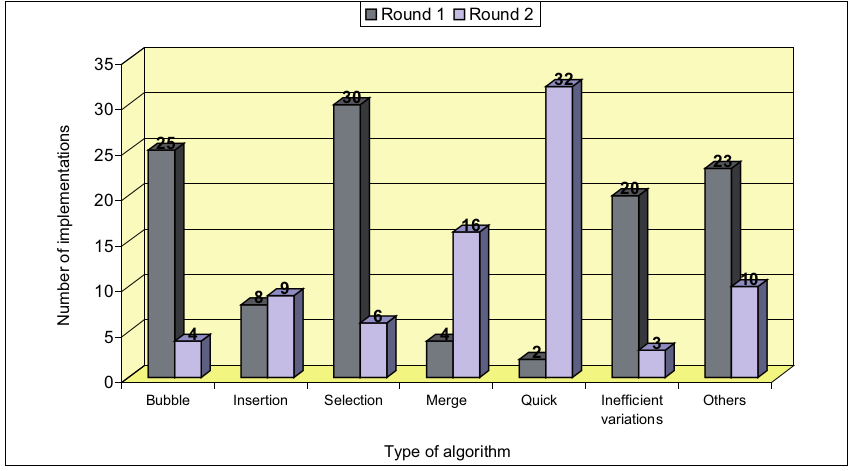
\includegraphics[scale=0.4]{imagem/clusterManual.png}
        \caption{Agrupamento manual das implementações dos estudos estudantes no
        	primeiro e segundo \textit{round}}
        \label{fig:clusterManual}
    \end{figure}
    
    Após o agrupamento manual dos métodos de ordenação implementados pelos alunos,
    \citeonline{Taherkhani:2012} realizou o reconhecimento automático das
    implementações por meio da ferramenta Aari. Inicialmente a ferramenta foi
    treinada para reconhecer os algorítmos de ordenação: \textit{bubble sort},
    \textit{insertion sort}, \textit{selection sort}, \textit{mergesort} e
    \textit{quicksort}. A Figura \ref{fig:clusterAutomatico} apresenta o gráfico
    no qual o eixo x indica o algoritmo de ordenação e o eixo y indica a
    quantidade de implementações realizadas. Para cada algoritmo há duas colunas:
    a primeira coluna indica a quantidade de implementações que foram realizadas
    pelos alunos; e a segunda coluna representa a quantidade de implementações
    reconhecidas corretamente pela ferramente. A coluna \textit{Inefficient variations}
    foi gerada como consequência de modificações realizadas pelos alunos na
    estrutura de qualquer algoritmo de ordenação e essas variações foram
    consideradas como ineficiente, enquanto a coluna \textit{Others}, foi
    criada a partir das implementações de outros métodos de ordenação que
    não são citadas anteriormente. Nota-se que todas os métodos de ordenação
    \textit{selection sort} e \textit{quicksort} foram classificados corretamente.
    
    \begin{figure}[ht]
        \centering
        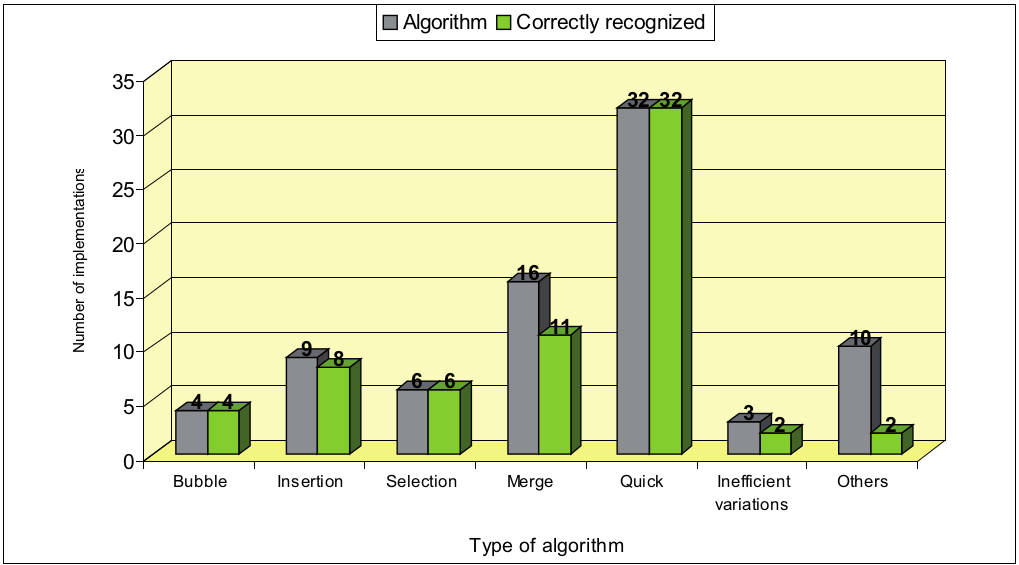
\includegraphics[scale=0.33]{imagem/clusterAutomatico.png}
        \caption{Comparação das implementações dos alunos dos \textit{clusters}
        	manual e automático do \textit{Round} 2}
        \label{fig:clusterAutomatico}
    \end{figure}
    
    \citeonline{Glassman:2015} apresentam o OverCode (Figura \ref{fig:interfaceOverCode}),
    ferramenta para visualização de informação no qual demonstra os clusters formados,
    as principais instruções utilizadas pelas implementações presentes em um
    determinado agrupamento e as linhas de código de uma determinada função/método.
    A ferramenta é voltada para aqueles que realizarão a validação das submissões.
    
    Após a clusterização dos códigos fontes, é realizado uma limpeza de código,
    no qual é retirado todas as linhas em branco do código gerando o código limpo,
    tornando-o legível, executável e descrito na ferramenta. Como um \textit{cluster}
    é um conjunto de várias soluções, pode ocorrer das soluções, mesmo semelhantes,
    possuam variáveis diferentes. Por isso criou-se uma ferramente de reescrita
    para poder renomear as variáveis de um algoritmo por meio da interface,
    seguindo regras que foram encontradas durante os testes com os primeiros protótipos.
    
    OverCode também registra os valores que uma determinada variável assume como
    um teste de mesa. Entretanto, tal funcionalidade foi retirada, pois alguns
    usuários pilotos o classificaram como confuso. Outra utilidade realizada pela
    análise da execução do programa (trace) é a identificação de variáveis idênticas
    que são encontradas a partir da análise das sequências de variáveis, assim, se
    duas variáveis com nomes diferente, possuem os mesmos valores durante o
    \textit{trace}, elas são consideradas variáveis idênticas.
    
    Por fim, os autores concluíram que a interface auxilia os assistentes de
    ensino a terem uma visão de alto nível dos alunos, podendo compreender os
    erros e fornecer um \textit{feedback} mais relevante, devido a clusterização
    das implementações, visto que diminui consideravelmente a quantidade de
    projetos a serem corrigidos.
    
    \begin{figure}[ht]
        \centering
        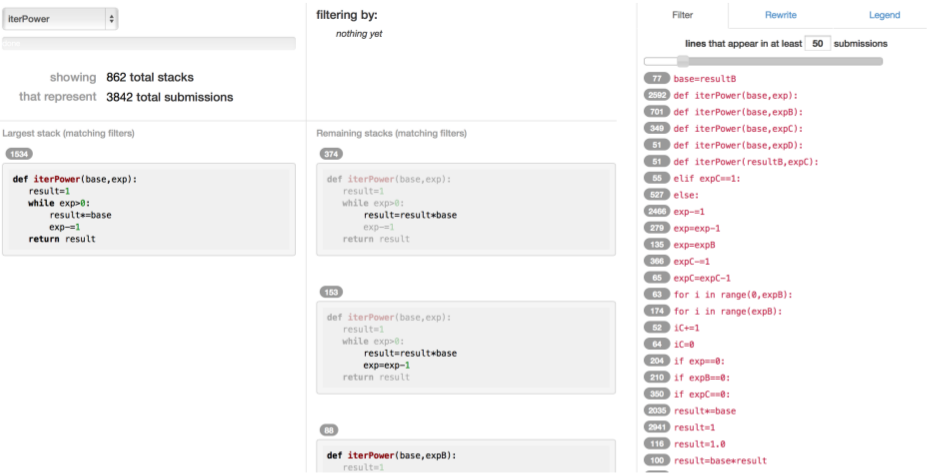
\includegraphics[scale=0.4]{imagem/overCode.png}
        \caption{Interface OverCode. A coluna a esquerda mostra dois painéis, o
        	primeiro painel apresenta o número de agrupamentos, nesse caso, as
        	pilhas, e o número total de submissões, enquanto o segundo painel,
        	mostra a maior pilha. A coluna central apresenta: a opção de busca,
        	filtrando por uma determinada palavra no quadro superior; e as pilhas
        	remanescentes no quadra inferior. Enquanto a terceira coluna apresenta
        	a frequência com que as linhas de códigos estão presentes nas soluções}
        \label{fig:interfaceOverCode}
    \end{figure}
    
    É utilizado o conceito de pilhas para representar os agrupamentos, desta forma,
    a comparação das pilhas menores com a pilha maior ocorre entre a primeira e a
    segunda coluna dando ênfase nas linhas que estão implementadas diferentes. Com
    isso, é possível verificar como cada pilha foi montada e a característica daquela
    pilha quando comparada com a pilha maior. Como utiliza análise dinâmica para
    classificar as submissões, é possível verificar o \textit{traceback} da
    variável que desejar ao longo de sua execução em um caso de teste a fim de
    auxiliar os usuários a entenderem a execução do algoritmo.
    
    \citeonline{Wei2015} apresenta uma ferramenta para auxiliar na correção das
    submissões dos MOOC's de forma a agrupar pedaços (\textit{chuncks}) de códigos
    fontes semelhantes, agrupá-los conforme sua similaridade e alocar cada conjunto
    de implementações ao estudante com conhecimento suficiente para revisá-los.
    
    Foi necessário realizar o particionamento do código para torná-lo legível
    e fácil de compreender, os pedaços foram extraídos das implementações como
    se fossem funções, entretanto, há uma dificuldade para verificar as submissões
    quando ocorria uma chamada de função em uma outra função, dificultando a divisão
    em pedaços do código. Também foi necessário normalizar cada submissão a fim de
    encontrar o estilo de escrita, visto que até mesmo o nome da variável pode
    alterar o estilo de escrita.
    
    A ferramenta\cite{Wei2015} normaliza o código por meio de três regras:
    \begin{enumerate}
    	\item Remoção de espaços, linhas em branco e comentários;
    	\item Exclusão de palavras reservadas da linguagem de programação,
    	identificadores predefinidos e nomes de funções de bibliotecas;
    	\item E substituição dos identificadores de variáveis do usuário por um
    	símbolo especial.
    \end{enumerate}
    Com isso foi calculado um valor \textit{hash} para cada \textit{substring}
    do código a fim de verificar a similaridade do estilo de escrita \textit{token}
    a \textit{token} e utilizado o algoritmo de \texttt{winnowing} para escolher
    o menor subconjunto do estilo de escrita a fim de realizar as comparações
    por meio do coeficiente de similaridade de \textit{Jaccard}. E com a finalidade
    de identificar a dificuldade da implementação, foi utilizado a distância
    Euclidiana para comparar as características extraídas - quantidade de métodos
    invocados e laços de repetição aninhados - e o \textit{K Nearest Neighbor}
    (\texttt{k-NN}) para identificar o nível de dificuldade de revisão do
    \textit{chunck}.
    
	\begin{figure}
		\centering
		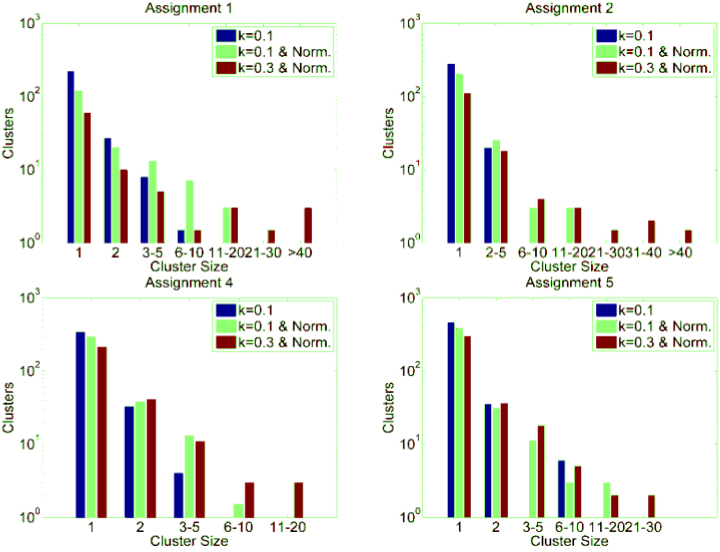
\includegraphics[width=0.7\linewidth]{imagem/clusteringPerformance}
		\caption{Distribuição do agrupamentos. A barra azul representa o agrupamento
			sem normalização, enquanto as barras verde e vermelho possuem o valor
			de \textit{k} diferente, entretanto, ambas estão normalizadas. O
			\textit{cluster size} é referente ao tamanho dos pedaços e os
			\textit{clusters} representa o número de agrupamentos.}
		\label{fig:clusteringPerformance}
	\end{figure}
    
	Conforme a Figura \ref{fig:clusteringPerformance} pode-se notar que a
	distribuição dos \textit{chuncks} sem normalização de código é inadequado,
	visto que vários pedaços nas atribuições 2 e 4 estavam sozinhos, e o maior
	agrupamento possuía apenas 3 pedaços. Enquanto a tarefa 1 e 2 apresentou
	bons agrupamentos e o tamanho dos grupos era condizente com a quantidade de
	estudantes (200) quando \textit{k} era igual a 3.0. As tarefas 4 e 5 não foram
	satisfeitas devido ao total de pedaços em um grupo ser próximo de 20 e o
	restante dos códigos foram pequenos agrupamentos.
	
	É possível notar que tal abordagem não obteve sucesso, pois, independente da
	tarefa selecionada, nota-se que a maioria dos \textit{clusters} formados
	possuíam apenas um pedaço de código. Com isso pode-se aumentar o tempo de
	correção das submissões, visto que uma implementação completa pode gerar um
	ou mais pedaços de código, dificultando a revisão da submissão e podendo tomar
	um tempo maior para que fosse realizado um \textit{feedback} preciso para o
	estudante.